\documentclass[a4paper,11pt]{jsarticle}

% 数式
\usepackage{amsmath,amsfonts}
\usepackage{amsthm}
\usepackage{bm}
\usepackage{mathtools}
\usepackage{amssymb}

% 表
\usepackage[utf8]{inputenc}
\usepackage{diagbox} % 斜線付きセルを作成するために必要
\usepackage{booktabs} % 表の罫線を美しくするために必要
\usepackage{hhline} % 水平罫線を制御するために必要

% 画像
\usepackage[dvipdfmx]{graphicx}
\usepackage{ascmac}
\usepackage{physics}
\usepackage{float} % 追加

% 図
\usepackage[dvipdfmx]{graphicx}
\usepackage{tikz} %図を描く
\usetikzlibrary{positioning, intersections, calc, arrows.meta,math} %tikzのlibrary

% ハイパーリンク
\usepackage[dvipdfm,
  colorlinks=false,
  bookmarks=true,
  bookmarksnumbered=false,
  pdfborder={0 0 0},
  bookmarkstype=toc]{hyperref}

% 式番号を章ごとにリセット
\numberwithin{equation}{section}

\begin{document}

\title{9章}
\author{大上由人}
\date{\today}
\maketitle

\section*{9.1}
\subsection*{9.1.1}
Maxwellの悪魔と呼ばれる思考実験について考察する。初め左右の部屋が等温である系について、粒子の測度が速いものと遅いものを区別するdemonがいるとする。このとき、demonは、粒子の速いものを一方の部屋に、遅いものをもう一方の部屋に分けることができる。
そうすると、最終的に左右の部屋の温度が異なる状態になり、系のエントロピーが減少するように思われる。
\begin{figure}[H]
    \begin{center}
    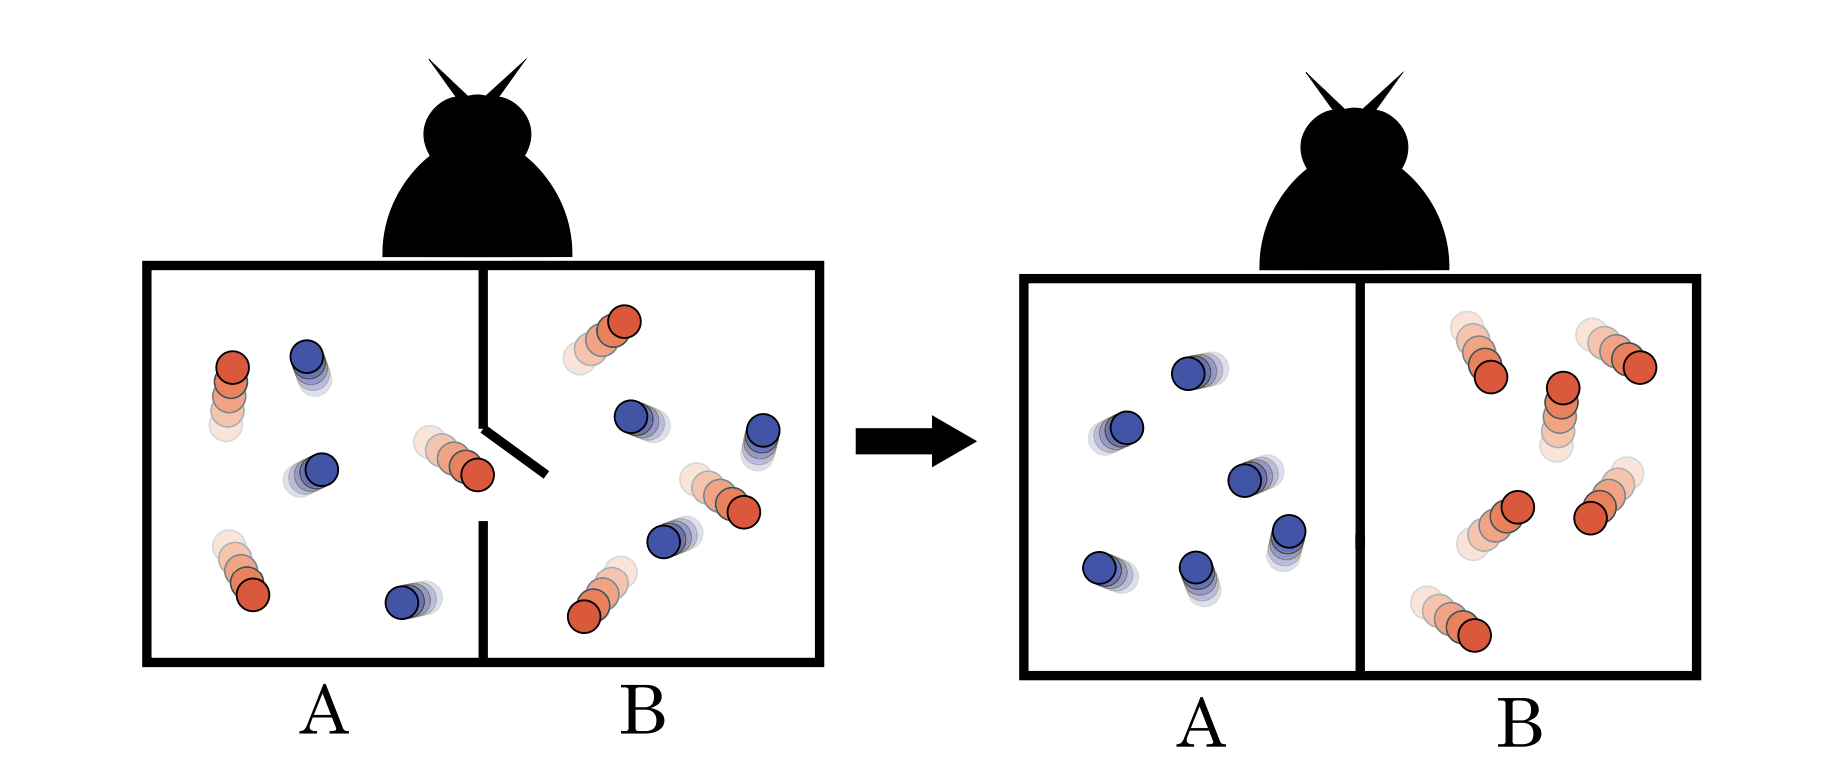
\includegraphics[width=100mm]{demon.png}
    \end{center}
    \caption{Maxwellの悪魔}
    \label{fig:Maxwelldemon}
\end{figure}

\subsection*{9.1.2}
Maxwellの悪魔を単純化したものとして、シラードエンジンとよばれる等温サイクルを考察する。シラードエンジンの過程は以下の通りである。\\
\begin{figure}[H]
    \begin{center}
    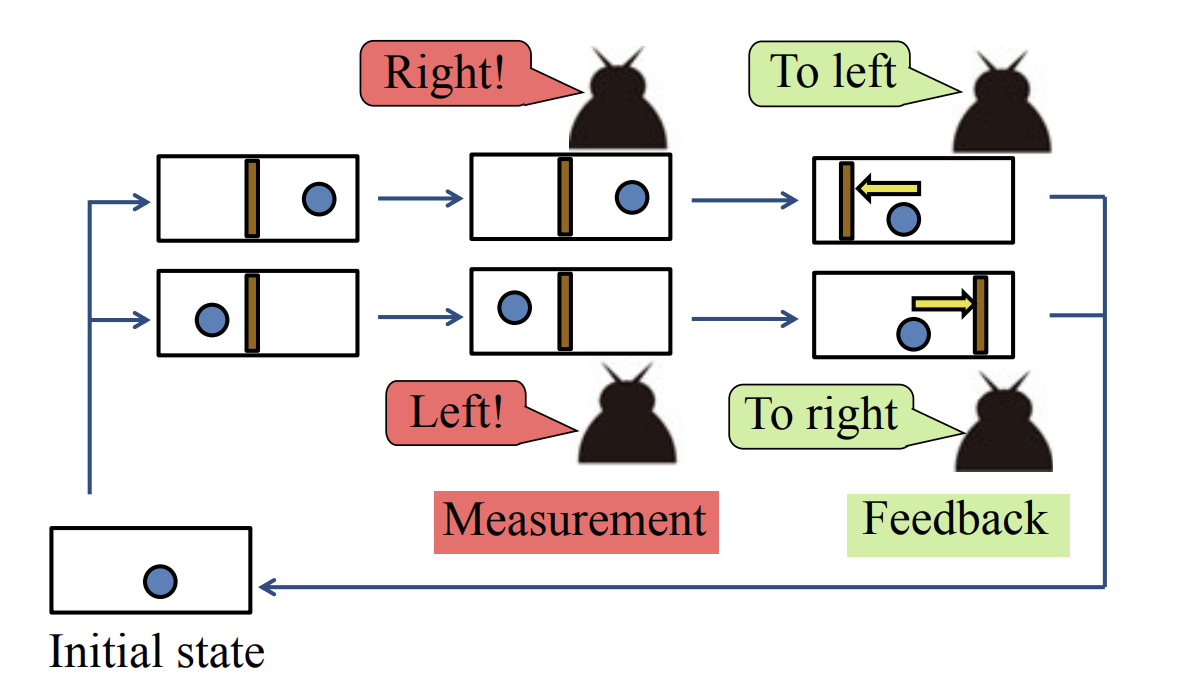
\includegraphics[width=100mm]{Szilard.png}
    \end{center}
    \caption{Szilard engine}
    \label{fig:Szilard}
\end{figure}
着目系は1粒子理想気体であるとする。過程は以下の通りである。
\begin{enumerate}
    \item 粒子が容器全体に存在し得る状態から始める。
    \item demonが、系にしきりを入れる。このとき、粒子は左右のどちらかに入り、demonは、粒子がどちらにいるかを確認する。(measurement)
    \item 粒子のない方向にしきりを動かす。(feedback)
    \item 壁を取り除く(初期状態に戻る)。
\end{enumerate}
このとき、3つ目の過程で仕事をとりだすことができる。とくに、系のちょうど半分にしきりを設けるとき、この仕事は、
\begin{equation}
    W_{\text{ext}} = \int_{\frac{V}{2}}^V PdV = \int_{\frac{V}{2}}^V \frac{kT}{V}dV = kT\log 2
\end{equation}
となる。この結果は、一見すると、マクロ系の熱力学におけるKelvinの原理に反するように思える。
\footnote{
    Kelvinの原理は、任意の等温サイクルにおいて、
    \begin{equation}
        W_{\text{ext}} \leq 0
    \end{equation}
    であるという原理であった。
}
Szilardは、測定過程を熱機関と測定装置を結び付ける過程と考え、feedback過程をその結びつきを消費するものとして考えた。それを踏まえて、熱力学第二法則に反しないためには、
測定によるエントロピー生成が以下の不等式を満たす必要があると考えた:
\begin{equation}
    e^{-\frac{\bar{S_1}}{k}} + e^{-\frac{\bar{S_2}}{k}} \leq 1 \label{eq:9.1}
\end{equation}
ここで、$\bar{S_1}$は、粒子が領域1にいるときの平均エントロピー生成、$\bar{S_2}$は、粒子が領域2にいるときの平均エントロピー生成である。\\
\textbf{(\ref{eq:9.1})式の導出}\\
$p_i = \frac{V_i}{V}$を粒子が領域iにいる確率とする。初め、粒子は容器の全体に存在し得るので、エントロピーは
\begin{align}
k\log V + \text{const.}
\end{align}
である。同様に粒子が領域1,2にいるときのエントロピーは、それぞれ、
\begin{align}
    S_1 &= k\log V_1 + \text{const.} \\
    S_2 &= k\log V_2 + \text{const.}
\end{align}
である。よって、系の平均エントロピー変化は、
\begin{align}
    \bar{s} &=p_1k(\log V_1 - \log V) + p_2k(\log V_2 - \log V) \\
    &= k(p_1\log p_1 + p_2\log p_2)
\end{align}
となる。また、測定による平均エントロピー生成は、
\begin{align}
    \bar{S} = p_1\bar{S_1} + p_2\bar{S_2}
\end{align}
である。全系についての熱力学第二法則は、
\begin{align}
    \bar{S} + \bar{s} &= p_1\bar{S_1} + p_2\bar{S_2} + k(p_1\log p_1 + p_2\log p_2) \geq 0
\end{align}
である。ここで、左辺を最小化することを考える。これは、ラグランジュの未定乗数法を用いて、
\begin{align}
    p_1\bar{S_1} + p_2\bar{S_2} + k(p_1\log p_1 + p_2\log p_2) + k\lambda(1-p_1-p_2)
\end{align}
を最小化することと等価である。$p_1,p_2,\lambda$についてそれぞれ偏微分すると、
\begin{align}
    &\bar{S_1} +k\log p_1 - k + k\lambda = 0 \\
    &\bar{S_2} +k\log p_2 - k + k\lambda = 0 \\
    &1-p_1-p_2 = 0
\end{align}
となる。これを変形して、
\begin{align}
    p_1 &= \exp(\lambda - \frac{\bar{S_1}}{k}) \\
    p_2 &= \exp(\lambda - \frac{\bar{S_2}}{k})
\end{align}
となる。これを用いて、
\begin{align}
    \lambda e^{\lambda}(e^{-\frac{\bar{S_1}}{k}} + e^{-\frac{\bar{S_2}}{k}}) \geq 0
\end{align}
となる。これより$\lambda \geq 0$であることがわかる。ここで、
\begin{align}
    p_1 + p_2 &= \exp(\lambda - \frac{\bar{S_1}}{k}) + \exp(\lambda - \frac{\bar{S_2}}{k}) = 1
\end{align}
より、
\begin{align}
    e^{-\frac{\bar{S_1}}{k}} + e^{-\frac{\bar{S_2}}{k}}  = e^{-\lambda} \leq 1
\end{align}
となる。よって、(\ref{eq:9.1})式が導かれる。\hfill\qedsymbol\\

\textbf{具体的なメモリーの導入}\\
Szilardは、(\ref{eq:9.1})式を満たすようなメモリーも導入した。以下ではその概要を見る。\\

\begin{figure}[H]
    \centering
\begin{tikzpicture}
    % Drawing the energy levels
    \draw[thick] (0,0) -- (1,0);
    \draw[thick] (0,2) -- (1,2);
    \draw[thick] (1.5,2) -- (2.5,2);
    \draw[thick,dotted] (3,2) -- (4,2);
    \draw[thick] (4.5,2) -- (5.5,2);
    
    % Label for degenerate levels
    \node at (2.5,2.5) {$g$個};
    \node at (-0.5,2) {$B$};
    \node at (-0.5,0) {$A$};
    
    % Energy axis
    \draw[->] (6.1,0) -- (6.1,3) node[anchor=west] {E};
    \draw (6.1,0) -- (5.9,0) node[anchor=east] {0};
    \draw (6.1,2) -- (5.9,2) node[anchor=east] {u};
\end{tikzpicture}
\caption{メモリーのエネルギー準位}
\label{fig:memory}
\end{figure}
図\ref{fig:memory}のような系を考える。1つのエネルギー準位が0であり、他のg個のエネルギー準位がuであるとする。エネルギーが低い準位、高い準位をそれぞれA,Bとする。
初期状態における温度を$T_0$とする。系の状態が$x =1,2$のとき、メモリーの温度を$T_A,T_B$とする。ただし、$T_A <T_0<T_B$であるとする。\\
このとき、メモリーの平均エネルギーは、
\begin{align}
    \bar{u}(T) = uq(T) = \frac{uge^{-\frac{u}{kT}}}{1+ge^{-\frac{u}{kT}}}
\end{align}
である。このとき、測定によるエントロピー生成とメモリー消去によるエントロピー生成の合計は、
\begin{align}
    S_i = \frac{\bar{u}(T_i)-\bar{u}(T_0)}{T_0} + \int_{T_i}^{T_0}\frac{1}{T}\frac{\dd \bar{u}(T)}{\dd T}\dd T
\end{align}
である。第一項がメモリー消去、第二項が測定によるエントロピー生成である。これを整理すると、%TODO: ここから先を書く
\begin{align}
    S_i = k\left(q(T_i)\log\frac{q(T_i)}{q(T_0)} + p(T_i)\log\frac{p(T_i)}{p(T_0)}\right)
\end{align}
となる。ただし、
\begin{align}
    q(T) &= \frac{1}{1+ge^{-\frac{u}{kT}}} \\
    p(T) &= \frac{ge^{-\frac{u}{kT}}}{1+ge^{-\frac{u}{kT}}}
\end{align}
である。\\
\textbf{(\ref{eq:9.1}式の導出)}\\
\begin{align}
    S_i &= \frac{\bar{u}(T_i)-\bar{u}(T_0)}{T_0} + \int_{T_i}^{T_0}\frac{1}{T}\frac{\dd \bar{u}(T)}{\dd T}\dd T \\
    &= \frac{\bar{u}(T_i)-\bar{u}(T_0)}{T_0} + \int_{T_i}^{T_0}\left(\dv{T} \left(\frac{\bar{u}(T)}{T} +k\log(1+ge^{-\frac{u}{kT}})\right)\right)\dd T \\
    &= \frac{\bar{u}(T_i)-\bar{u}(T_0)}{T_0} + \left(\frac{\bar{u}(T_0)}{T_0} +k\log(1+ge^{-\frac{u}{kT_0}})\right) - \left(\frac{\bar{u}(T_i)}{T_i} +k\log(1+ge^{-\frac{u}{kT_i}})\right) \\
    &= \bar{u}(T_i)\left(\frac{1}{T_0} - \frac{1}{T_i}\right) + k\log\frac{1+ge^{-\frac{u}{kT_0}}}{1+ge^{-\frac{u}{kT_i}}} \\
    &= q(T_i)\left(\frac{u}{T_0} - \frac{u}{T_i}\right) + k\log\frac{p(T_i)}{p(T_0)} \quad \because \frac{1}{p(T)} = 1+ge^{-\frac{u}{kT}}\\
    &= q(T_i)\left(-k\log\frac{q(T_0)}{p(T_0)}\right) + k\log\frac{q(T_i)}{p(T_i)} + k\log\frac{p(T_i)}{p(T_0)} \\
    &= q(T_i)k\log\frac{p(T_0)}{q(T_0)}\frac{q(T_i)}{p(T_i)} + k\log\frac{p(T_i)}{p(T_0)} \\
    &= q(T_i)k\log\frac{q(T_i)}{q(T_0)} - q(T_i)k\log\frac{p(T_i)}{p(T_0)} + k\log\frac{p(T_i)}{p(T_0)} \\
    &= q(T_i)k\log\frac{q(T_i)}{q(T_0)} + p(T_i)k\log\frac{p(T_i)}{p(T_0)} \quad \because p(T) + q(T) = 1\\
    &= k\left(q(T_i)\log\frac{q(T_i)}{q(T_0)} + p(T_i)\log\frac{p(T_i)}{p(T_0)}\right)
\end{align}
により、(\ref{eq:9.1})式が導かれる。\hfill\qedsymbol\\

これの極限を考える。$T_A \to 0,g \to \infty$とすると、$p(T_A) = q(T_B) = 1, p(T_B) = q(T_A) = 0$となる。よって、
\begin{align}
    & S_A = -k\log p(T_0) \\
    & S_B = -k\log q(T_0)
\end{align}
となる。これは、(\ref{eq:9.1})式の等号が成り立つときのエントロピー生成である。\\

\subsection*{9.1.3}
Brillouin、Gaborの議論についてみる。\\
Brillouinは、光を用いて粒子の位置を測定することを考えた。光が粒子に当たると光が散乱し、そのエネルギーが熱に変わる。測定結果を見るには$h\nu \gg kT$である必要がある。(背景輻射との区別をするため。)
このとき、測定過程におけるエントロピーが、feedback過程で取り出される仕事よりも大きくなることを主張した。\\

また、Gaborも光を用いて粒子の位置を測定することを考えた。

箱の中に単一の粒子が入っている。ある$X>1$を固定し、粒子が箱の底の$\frac{1}{X}$の範囲にいるかどうかを考える。粒子がこの領域の中に入っていたら、箱の底と上側とを分離する壁を挿入する。
壁が挿入されると、粒子のエントロピーは$kT\log X$だけ減少する。Gaborは、この測定には少なくとも$\frac{X}{2}$個の光子が必要であると考えた。このとき、$\frac{Xh\nu}{2} $以上のエネルギーが散乱される(これは、エントロピーによる利得$kT\log X$よりもはるかに大きい)。\\

\subsection*{9.1.4}
LandauerおよびBennettの議論についてみる。彼らは、メモリー消去にかかるコストに注目した。\\

\begin{figure}
    \begin{center}
    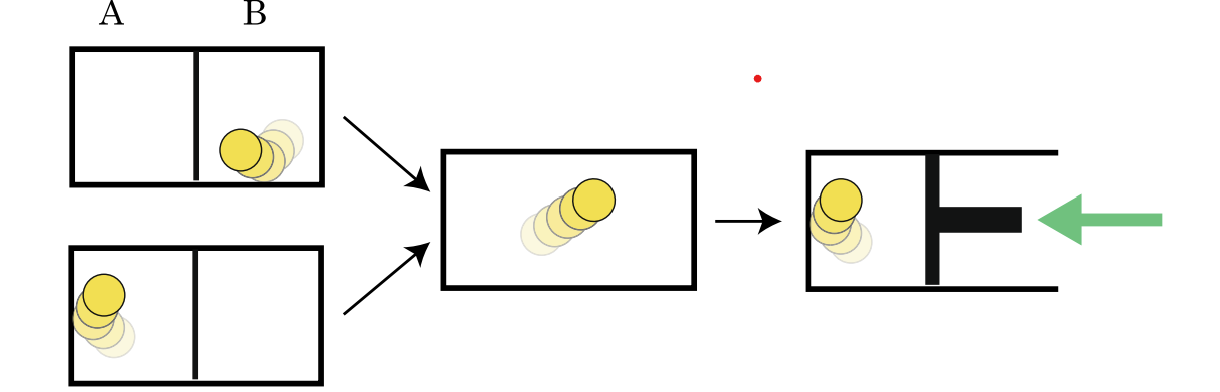
\includegraphics[width=100mm]{Landauer.png}
    \end{center}
    \caption{Landauerの原理}
    \label{fig:Landauer}
\end{figure}

メモリー消去は、消去前の状態によらず、一意な状態になる。このとき、シャノンエントロピーが減少する。シャノンエントロピーが減少することが熱放出と結びついていると考えた(Landauerの原理)。\\

Bennettもmemory消去にかかるコストに注目した。彼は以下のような具体例を構成した。\\
\begin{figure}[H]
    \begin{center}
    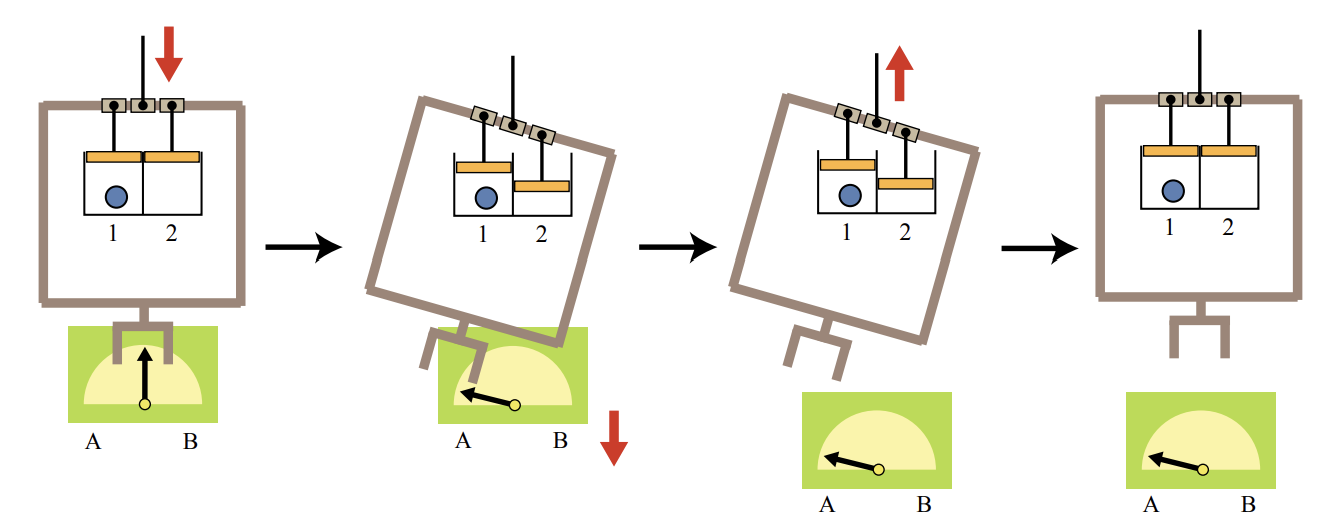
\includegraphics[width=100mm]{Bennett.png}
    \end{center}
    \caption{Bennettの議論}
    \label{fig:Bennett}
\end{figure}
\begin{enumerate}
    \item ピストンを準静的に下げ、engineの状態を記録する。(この過程では仕事が必要)
    \item メモリー消去を行い、ピストンを準静的に上げる。(この過程では、一つ前と同じだけの仕事を取り出すことができる)
\end{enumerate}
これはBrillouinの議論の反例である。\\

\subsection*{9.1.5}
Maxwell demonの問題は、engineとmemoryの相関が大事であり、メモリー消去が大事なわけではないということを言っている。

\section*{9.2}
\subsection*{9.2.1}
二つの確率変数の相関を測る指標として、相互情報量を導入する。\\
\begin{itembox}[l]{\textbf{Def:相互情報量}}
    二つの確率変数$x,y$について、その相互情報量$I(x,y)$は、
    \begin{align}
        I(x,y) = \sum_{i,j}P(x_i,y_j)\log\frac{P(x_i,y_j)}{P(x_i)P(y_j)}
    \end{align}
    で定義される.

\end{itembox}
このとき、シャノンエントロピーの定義と見比べることで、
\begin{align}
    I(x,y) = H(x) - H(x|y) = H(y) - H(y|x)
\end{align}
であることがわかる。\\%TODO: ここの計算しておく
$(\because$)\\
定義から、
\begin{align}
    H(x|y) &= -\sum_{i,j}P(x_i,y_j)\log P(x_i|y_j) \\
    H(x) &= -\sum_{i}P(x_i)\log P(x_i)
\end{align}
である。よって、
\begin{align}
    I(x,y) &= \sum_{i,j}P(x_i,y_j)\log\frac{P(x_i,y_j)}{P(x_i)P(y_j)} \\
    &= \sum_{i,j}P(x_i,y_j)\log \frac{P(x_i|y_j)P(y_j)}{P(x_i)P(y_j)} \\
    &= \sum_{i,j}P(x_i,y_j)\log \frac{P(x_i|y_j)}{P(x_i)} \\
    &= \sum_{i,j}P(x_i,y_j)\log \frac{P(x_i,y_j)}{P(x_i)} \\
    &= H(x) - H(x|y)
\end{align}
である。\hfill\qedsymbol\\
この式を見ると、相互情報量は、$y$の値を知ることによる、エントロピーの減少量と解釈することができる。\\
今、
\begin{align}
    I(x,y) = H(x) - H(x|y) \geq 0
\end{align}
であるから、相互情報量は、常に非負である。とくに、$x,y$が独立であるとき、
\begin{align}
    I(x,y) = 0
\end{align}
である。これは、$y$の値を知っても、$x$の値に関する情報が何も得られないことに対応している。\\

また、確率的な相互情報量も導入しておく。
\begin{itembox}[l]{\textbf{Def:確率的相互情報量}}
        確率的相互情報量$\hat{I}(x,y)$は、
        \begin{align}
                \hat{I}(x,y) = \log\frac{P(x,y)}{P(x)P(y)}
        \end{align}
        で定義される.

\end{itembox}
確率的相互情報量の期待値は、相互情報量と等しい。\\

\subsection*{9.2.2}
$X$と$Y$の複合系を考える。この節では、$X$のみが、$Y$に依存して時間発展することができ、$Y$は時間発展しないとする。
初め、$X$と$Y$は相関があってもよいとする。\\
初期状態及び終状態の相互情報量を、$I_{\text{i}},I_{\text{f}}$とする。また、初期状態および終状態の系$X,Y$のエントロピーを、それぞれ、$S_{X\text{i}},S_{Y\text{i}},S_{X\text{f}},S_{Y\text{f}}$とする。\\
このとき、初期状態及び終状態の全系のシャノンエントロピーは、
\begin{align}
    S_{\text{tot,i}} &= S_{X\text{i}} + S_{Y\text{i}} - I_{\text{i}} \\
    S_{\text{tot,f}} &= S_{X\text{f}} + S_{Y\text{f}} - I_{\text{f}}
\end{align}
である。\\
%TODO: ここの計算をする
$(\because)$\\
相互情報量の定義から、
\begin{align}
    I_{\text{i}} &= \sum_{i,j}P_{\text{i}}(x_i,y_j)\log\frac{P_{\text{i}}(x_i,y_j)}{P_{\text{i}}(x_i)P_{\text{i}}(y_j)} \\
    &= \sum_{i,j}P_{\text{i}}(x_i,y_j)\log P_{\text{i}}(x_i,y_j) - \sum_{i,j}P_{\text{i}}(x_i,y_j)\log P_{\text{i}}(x_i) - \sum_{i,j}P_{\text{i}}(x_i,y_j)\log P_{\text{i}}(y_j) \\
    &= -S_{X\text{tot,i}}  + S_{X\text{i}} + S_{Y\text{i}}
\end{align}
である。終状態についても同様である。\hfill\qedsymbol\\


このとき、全系についての熱力学第二法則は、
\begin{align}
    \sigma_X = \Delta S_X +\beta Q_X \geq \Delta I
\end{align}
である。この関係は、沙川-上田関係とも呼ばれる。(9.3で導出する)\\
この関係は、相関の強さが変わったら、(たとえ片方が時間変化しないとしても)それに合わせて熱力学第二法則を修正する必要があるということである。シラードエンジンにおいては、$X$をメモリーに、$Y$を着目系に対応させると、この関係が成り立つことがわかる。\\

\subsection*{9.2.3}
沙川-上田関係を用いて、シラードエンジンについて考察する。\\
$W$を取り出されるエネルギーとして、エントロピー生成は、
\begin{align}
    \sigma = -\beta W + \Delta S
\end{align}
である。ここで、$\Delta S$は、エントロピーの変化である。また、測定過程のあとの相互情報を$I_{\text{mem}}$とする。\\
\textbf{測定過程}\\
しきりを入れたときに、AまたはBのどちらかに粒子が入り、メモリーのシャノンエントロピーが増加する。また、engineとメモリーの間に相関ができる。このときの沙川-上田関係は、engineが時間変化しないとして、
\begin{align}
    \ev{e^{-\hat{\sigma}_Y+\hat{I}_{\text{mem}}}} = 1
\end{align}
すなわち、
\begin{align}
    \sigma_Y \geq I_{\text{mem}}
\end{align}
である。\\

\textbf{feedback過程}\\
情報量が変わらないため、engineのエントロピーは変化しないのに対し、しきりを動かすため、外部に仕事を取り出すことができる。また、engineとメモリーが相関を失う。このときの沙川-上田関係は、memoryが時間変化しないとして、

\begin{align}
    \ev{e^{-\hat{\sigma}_X-\hat{I}_{\text{mem}}}} = 1
\end{align}
すなわち、
\begin{align}
    \sigma_X \geq -I_{\text{mem}}
\end{align}
である。\\

\textbf{メモリーの消去}\\
粒子がどちらにいたかの情報をリセットするので、その分メモリのシャノンエントロピーが減少する。また、メモリをもとの状態に戻すために外部から仕事をされる。このときの沙川-上田関係は、
\begin{align}
    \ev{e^{-\hat{\sigma}_Y}} = 1
\end{align}
すなわち、
\begin{align}
    \sigma_Y \geq 0
\end{align}
である。\\

これまでの過程をまとめると、以下の図のようになる。\\
\begin{figure}[H]
    \begin{center}
    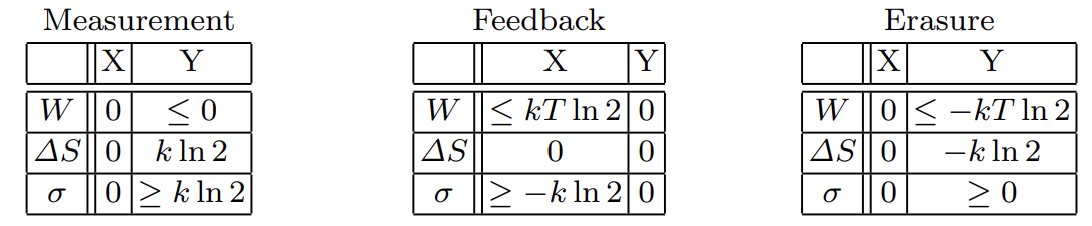
\includegraphics[width=100mm]{mfe.png}
    \end{center}
    \caption{Szilard engine}
    \label{fig:mfe}
\end{figure}
上の議論からわかるように、熱力学第二法則に修正が必要なのは、測定過程とfeedback過程である。メモリー消去の過程については、普通の熱力学と同じである。このことを踏まえると、メモリー消去を含まないようなシラードエンジンを構成することができる。
このサイクルをまとめると以下のようになる。\\
\begin{figure}[H]
    \begin{center}
    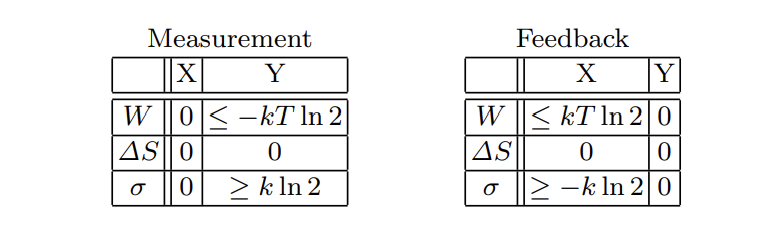
\includegraphics[width=100mm]{cycle.png}
    \end{center}
    \caption{メモリー消去を含まないようなシラードエンジン}
    \label{fig:cycle}
\end{figure}

\section*{9.3}
沙川-上田関係を導出する。\\
\subsection*{9.3.1}
\textbf{設定}\\
hogehoge

\begin{itembox}[l]{\textbf{Def:沙川-上田関係}}
    系$X$のエントロピー生成は以下の関係を満たす:
    \begin{align}
        \ev{e^{-\hat{\sigma}_X+\sum_{n=1}^N\Delta \hat{I}^{2n} }} = 1
    \end{align}
    ただし、hoge
\end{itembox}



\end{document}